\chapter{Interpretability}
\label{ch:IP}
\label{sec:interpret}

\section{Importance of Interpretability}
Interpretability refers to the capability to explain and understand how a model arrives at its predictions or decisions. Regression models and decision trees are simple to understand and, thus, very popular in the banking industry. On the contrary, more advanced machine learning models show a "Black Box" nature; their model logic and output are difficult to explain. Machine learning models' complex structures have advantages and disadvantages. While they can detect non-linear relationships and correlations and may show improved accuracy or efficiency, they are also prone to overfitting and lack explainability. Their "Black Box" nature stems from the model's numerous transformations of input variables, as well as their optimization process.\footnote{\cite{Roberts2022} p.~56}

\subsection{Regulatory and Legal Requirements}
\label{sec:ref_leg}

Interpretability enables compliance with regulations and consumer protection laws such as the Capital Requirements Regulation (CRR) and General Data Protection Regulation (GDPR). Data protection principles such as purpose limitation, data minimisation and limitation on automated decisions are evident obstacles for complex artificial intelligence models. In the Capital Requirements Regulation (CRR Article 144(1)(a)), a requirement of the PD model development is stated as:

\begin{quote}

\emph{(a) the institution's rating systems provide for a meaningful assessment of obligor and transaction characteristics, a meaningful differentiation of risk and accurate and consistent quantitative estimates of risk;}

\end{quote}

Regulations mandate that both model developers and users provide explanations for credit-related decisions to their customers. Modelers, along with internal and external auditors, are obligated to validate not only the model's structure but also its results, ensuring whether the model aligns with domain knowledge and expectations. Interpretability helps identify potential biases, data issues or model limitations. 

Additionally, an unexplainable model used in production increases operational risk, as it becomes challenging to assess potential consequences, such as bias or fairness, and verify the accuracy of results or detect system errors. To circumvent the constraints imposed by regulatory requirements and consumer protection laws, machine learning models may find application in areas where the model's structure and output are not of utmost priority, such as in the collection process or fraud detection.\footnote{\cite{Roberts2022} pp.~57, 58} \footnote{\cite{Witzany:2017} p.~89}

\subsection{Data Management}
Before the development or deployment of machine learning models, a sound data management process must be established. The training data must be unbiased and accurately reflect the population the model will be deployed on, meaning that individual groups should not be over- or underrepresented. Failure to correct and validate the data utilized during the training phase or in production can yield unexpected outcomes or result in a biased model. Machine learning algorithms have the potential to amplify errors; as popular saying goes, "Garbage In - Garbage Out." \footnote{\cite{Roberts2022} p.~61}

\section{Methods for Interpretability Analysis}
Techniques to assess the interpretability of advanced models are also called model-agnostic explainability methods. They are algorithm-independent, usually applied after model development and assessed on global or local level, which means on data set or data observation level. Depending on the objective, the techniques can be allocated into five categories: feature importance, input variable impact, specific prediction analysis, output analysis and robustness check.\footnote{\cite{Roberts2022} p.~62}

\subsection{Feature Importance}
Feature importance measures the contribution of each variable in a predictive model to the overall model performance. If the performance drops significantly when changing the value of a variable while keeping other risk factors constant, it implies the importance of that particular feature. Relative feature importance compares the importance of features relative to each other, which helps prioritize features based on their influence on the model's predictions. To facilitate a meaningful comparison, the ranges of each variable need to be normalized to the same scale, enabling a direct assessment of their impact.\footnote{\cite{Roberts2022} p.~63}

\begin{figure}[H]
	\centering
	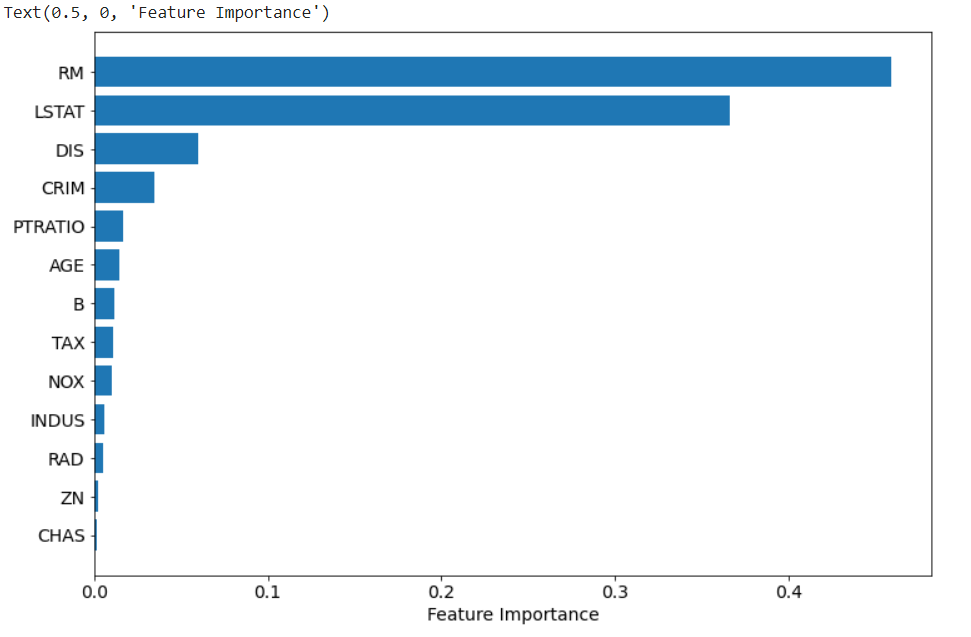
\includegraphics[width=0.625\textwidth]{./IN__featureimp.png}
    \caption{Feature Importance}
    \label{fig:in_featureimp}
\end{figure}

\subsection{Input Variable Impact}
Exploring the impact of individual variables is carried out through techniques like Partial Dependence Plots (PDP) and Individual Conditional Expectation (ICE), illustrated in Figure \ref{fig:in_pdp}. PDP visualizes the relationship between a specific feature and the model's predictions while holding other variables constant. They provide insights into the direction and magnitude of the feature's effect on default probability. ICE is an extension of PDP, illustrating how predictions change for an individual data point as a specific feature varies.\footnote{\cite{Roberts2022} p.~63}

\begin{figure}[H]
\begin{minipage}{.5\textwidth}
	\centering
	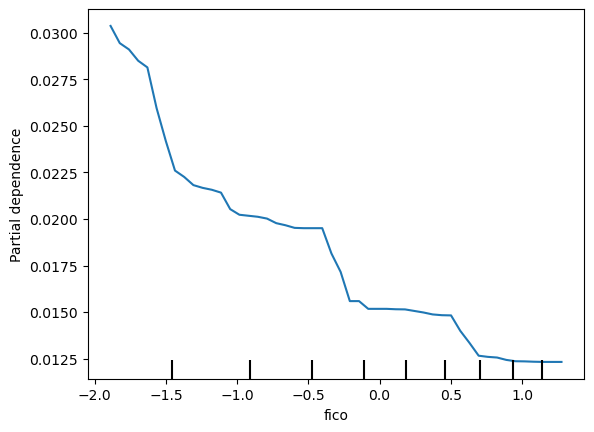
\includegraphics[width=0.9\textwidth]{./plot/ML/PDP_fico.png}
    \caption{Partial Dependence Plots}
    \label{fig:in_pdp}
\end{minipage}%
\begin{minipage}{.5\textwidth}
	\centering
	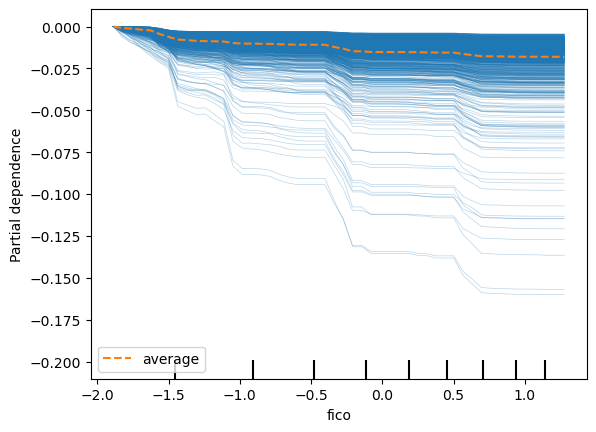
\includegraphics[width=0.9\textwidth]{./plot/ML/ICE_fico.png}
    \caption{Individual Conditional Expectation}
    \label{fig:in_ice}
\end{minipage}
\end{figure}

\newpage
\subsection{Individual Prediction Analysis}
For the interpretation of specific predictions, tools such as \ac{LIME} and Local rule-based explanations can be utilized. In the \ac{LIME} process, a local interpretable surrogate model is estimated. A small sample with similar variable values is selected and used to estimate a sparse linear regression model while using the predictions of the machine learning models as a target. Similarly, the Local rule-based explanations method builds a set of decision rules to act as a surrogate model in the interpretation process.\footnote{\cite{Roberts2022} p.~65-67}

\subsection{Output Analysis and Robustness Check}
During Counterfactual analysis, the feature values are slowly changed to assess which total changes are necessary to receive a specific prediction. Adversial testing is performed to analyze, how the machine learning model reacts to adversial attacks, which are input data deliberately designed with the aim of causing misclassification or incorrect output. 

Internal layers of Deep Neural Networks can be computed to detect adversial data to respond accordingly. Alternatively, adversial data can be incorporated in the development sample to include them during the training phase. 

In a sensitivity test, data with value ranges not captured by the training sample are used to analyze the model predictions and their performance beyond its training scope.\footnote{\cite{Roberts2022} p.~65-67}
